% Text summarization (T1): transcript -> speaker turns -> chunks -> map -> collapse -> reduce -> hearing summary.
% Parsing and chunking: chunking.py; map/collapse/reduce prompts: summarize.py (03_summarize_sst); assembly: 04_assemble_summaries.
% Generation only; the check against C-SPAN abstracts is not part of this chart.
% One column of wide blocks in three framed stages; block styles and legend as in T2.X and T3/TEMP/T3.X.
% Compile: pdflatex fig_text_summarization_flowchart.tex
\documentclass[border=8pt]{standalone}
\usepackage[T1]{fontenc}
\usepackage{tgtermes}
\usepackage{tikz}
\usetikzlibrary{positioning, shapes.symbols, shadows, arrows.meta, fit, backgrounds, calc}

% Figure Style Guide colors (S3)
\definecolor{RED}{HTML}{B31942}
\definecolor{BLUE}{HTML}{0A3161}
\definecolor{MIDNIGHTBLUE}{HTML}{004953}
\definecolor{GREY}{HTML}{A6A6A8}
\definecolor{BLACK}{HTML}{101820}
\colorlet{SUBTEXT}{GREY!35!BLACK}

% second line inside a block: the fact behind the block, in small dark grey
\newcommand{\sub}[1]{\\[1.5pt]{\scriptsize\color{SUBTEXT}#1}}

\begin{document}
\hyphenpenalty=10000 \exhyphenpenalty=10000
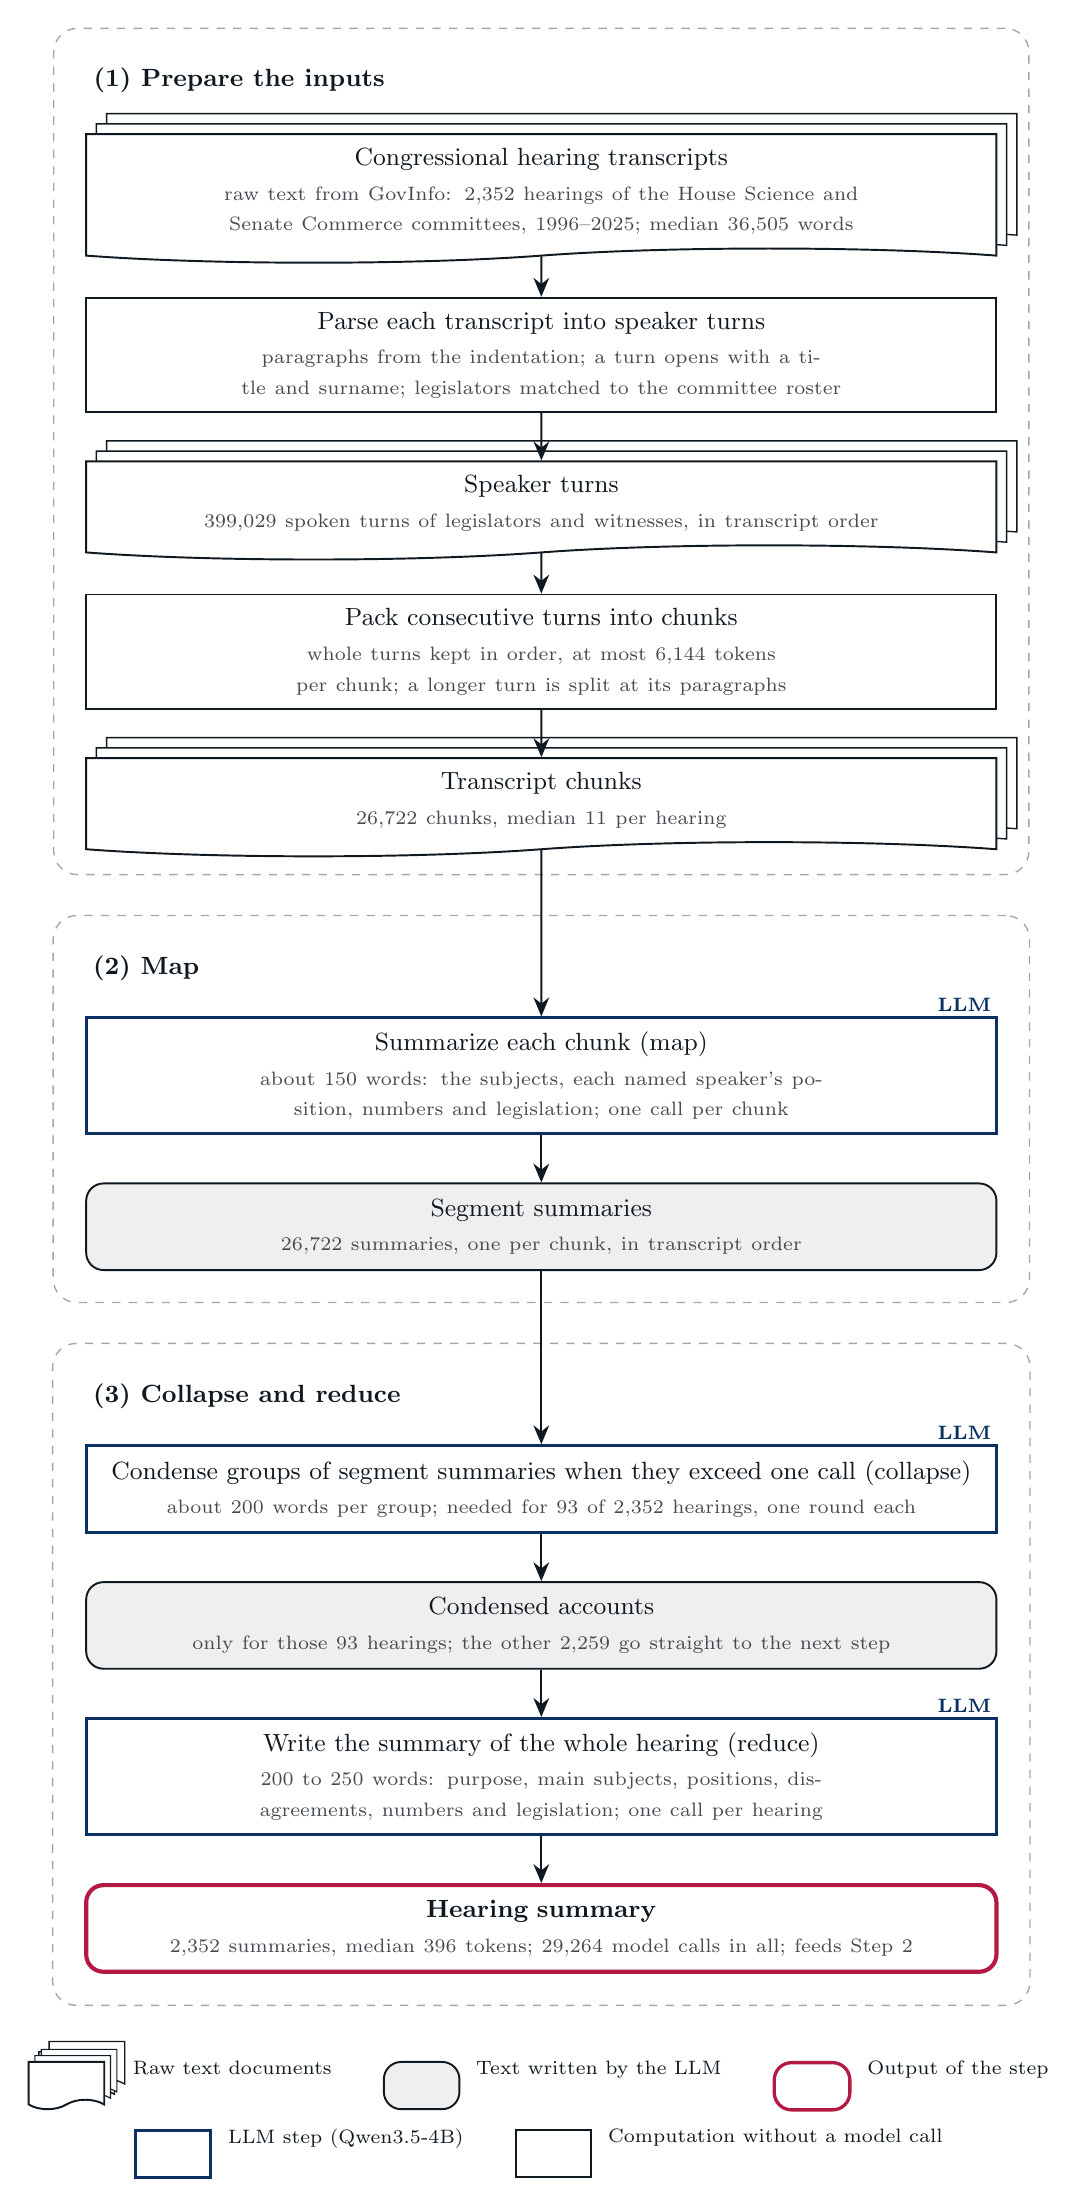
\begin{tikzpicture}[
  font=\small, text=BLACK, color=BLACK,
  node distance=6mm and 14mm,
  every node/.style={align=center},
  flow/.style={-{Stealth[length=2.4mm, width=2mm]}, line width=0.7pt, BLACK},
  % raw text: a stack of documents with a torn lower edge
  rawdoc/.style={tape, tape bend top=none, tape bend height=1.8mm, draw=BLACK, line width=0.7pt, fill=white,
                 text width=112mm, minimum height=12mm, inner sep=1.8mm,
                 double copy shadow={shadow xshift=1.3mm, shadow yshift=1.3mm, draw=BLACK, fill=white, line width=0.5pt}},
  % text written by the LLM: rounded, shaded
  summary/.style={rectangle, rounded corners=2.2mm, draw=BLACK, line width=0.7pt, fill=GREY!18,
                  text width=112mm, minimum height=11mm, inner sep=1.8mm},
  % LLM step: process box in BLUE with an LLM tag
  llm/.style={rectangle, draw=BLUE, line width=1.1pt, fill=white, text width=112mm, minimum height=11mm, inner sep=1.8mm,
              label={[text=BLUE, font=\scriptsize\bfseries, anchor=south east, inner sep=0pt, xshift=-0.8mm, yshift=0.5mm]north east:LLM}},
  % computation without a model call
  compute/.style={rectangle, draw=BLACK, line width=0.7pt, fill=white, text width=112mm, minimum height=11mm, inner sep=1.8mm},
  % data products of the step
  output/.style={rectangle, rounded corners=2.2mm, draw=RED, line width=1.5pt, fill=white, text width=112mm, minimum height=11mm, inner sep=1.8mm},
  lane/.style={draw=GREY, line width=0.5pt, dashed, rounded corners=3mm, inner sep=4mm},
  lanetitle/.style={font=\small\bfseries, text=BLACK, anchor=south west, inner sep=1mm},
]

% ---------------------------------------------------------------- (1) prepare the inputs
\node[rawdoc] (T1) {Congressional hearing transcripts\sub{raw text from GovInfo: 2,352 hearings of the House Science and Senate Commerce committees, 1996--2025; median 36,505 words}};
\node[compute, below=of T1] (T2) {Parse each transcript into speaker turns\sub{paragraphs from the indentation; a turn opens with a title and surname; legislators matched to the committee roster}};
\node[rawdoc, below=of T2] (T3) {Speaker turns\sub{399,029 spoken turns of legislators and witnesses, in transcript order}};
\node[compute, below=of T3] (T4) {Pack consecutive turns into chunks\sub{whole turns kept in order, at most 6,144 tokens per chunk; a longer turn is split at its paragraphs}};
\node[rawdoc, below=of T4] (T5) {Transcript chunks\sub{26,722 chunks, median 11 per hearing}};

% ---------------------------------------------------------------- (2) map
\node[llm, below=22mm of T5] (T6) {Summarize each chunk (map)\sub{about 150 words: the subjects, each named speaker's position, numbers and legislation; one call per chunk}};
\node[summary, below=of T6] (T7) {Segment summaries\sub{26,722 summaries, one per chunk, in transcript order}};

% ---------------------------------------------------------------- (3) collapse and reduce
\node[llm, below=22mm of T7] (T8) {Condense groups of segment summaries when they exceed one call (collapse)\sub{about 200 words per group; needed for 93 of 2,352 hearings, one round each}};
\node[summary, below=of T8] (T9) {Condensed accounts\sub{only for those 93 hearings; the other 2,259 go straight to the next step}};
\node[llm, below=of T9] (T10) {Write the summary of the whole hearing (reduce)\sub{200 to 250 words: purpose, main subjects, positions, disagreements, numbers and legislation; one call per hearing}};
\node[output, below=of T10] (T11) {\textbf{Hearing summary}\sub{2,352 summaries, median 396 tokens; 29,264 model calls in all; feeds Step 2}};

% ---------------------------------------------------------------- flows
\foreach \a/\b in {T1/T2, T2/T3, T3/T4, T4/T5, T5/T6, T6/T7, T7/T8, T8/T9, T9/T10, T10/T11}
  \draw[flow] (\a) -- (\b);

% ---------------------------------------------------------------- stage frames and titles
\node[lanetitle] (title1) at ([yshift=4mm]T1.north west) {(1) Prepare the inputs};
\node[lanetitle] (title2) at ([yshift=3.5mm]T6.north west) {(2) Map};
\node[lanetitle] (title3) at ([yshift=3.5mm]T8.north west) {(3) Collapse and reduce};
\begin{scope}[on background layer]
  \node[lane, fit=(title1)(T1)(T5)] {};
  \node[lane, fit=(title2)(T6)(T7)] {};
  \node[lane, fit=(title3)(T8)(T11)] {};
\end{scope}

% ---------------------------------------------------------------- legend
% Two matrix nodes, each anchored on the column's center line, so each legend row is centered under it.
\matrix[anchor=north, inner sep=0pt, column sep=1.2mm, row sep=0pt, nodes={inner xsep=0.8mm}] (legend1) at ($(T11.south)+(0,-11mm)$) {
  \node[rawdoc, text width=8mm, minimum height=6mm, inner sep=0.8mm, tape bend height=1.2mm,
        double copy shadow={shadow xshift=0.8mm, shadow yshift=0.8mm, draw=BLACK, fill=white, line width=0.4pt}] {}; &[1.5mm]
  \node[font=\scriptsize] {Raw text documents}; &[4.5mm]
  \node[summary, text width=8mm, minimum height=6mm, inner sep=0.8mm] {}; &
  \node[font=\scriptsize] {Text written by the LLM}; &[4.5mm]
  \node[output, text width=8mm, minimum height=6mm, inner sep=0.8mm, line width=1.2pt] {}; &
  \node[font=\scriptsize] {Output of the step}; \\
};
\matrix[anchor=north, inner sep=0pt, column sep=1.2mm, row sep=0pt, nodes={inner xsep=0.8mm}] (legend2) at ([yshift=-2mm]legend1.south) {
  \node[rectangle, draw=BLUE, line width=1.1pt, fill=white, text width=8mm, minimum height=6mm, inner sep=0.8mm] {}; &
  \node[font=\scriptsize] {LLM step (Qwen3.5-4B)}; &[4.5mm]
  \node[compute, text width=8mm, minimum height=6mm, inner sep=0.8mm] {}; &
  \node[font=\scriptsize] {Computation without a model call}; \\
};

\end{tikzpicture}
\end{document}
